%%%%%%%%%%%%%%%%%%%%%%%%%%%%%%%%%%%%%%%%%
% Beamer Presentation
% LaTeX Template
% Version 1.0 (10/11/12)
%
% This template has been downloaded from:
% http://www.LaTeXTemplates.com
%
% License:
% CC BY-NC-SA 3.0 (http://creativecommons.org/licenses/by-nc-sa/3.0/)
%
%%%%%%%%%%%%%%%%%%%%%%%%%%%%%%%%%%%%%%%%%

%----------------------------------------------------------------------------------------
% PACKAGES AND THEMES
%----------------------------------------------------------------------------------------

\documentclass[12pt,xcolor={dvipsnames}]{beamer}
%\setbeamersize{text margin left=1em,text margin right=1em}
\usepackage{mathtools}
\usepackage{amsmath}
\usepackage{bm}
\usepackage{hyperref}

\usepackage{graphicx} % Allows including images
\graphicspath{{/Users/rebecca/Documents/JER/MinimiseMatrixJER/MCvsData_PowhegPythia/}{/Users/rebecca/Documents/JER/MinimiseMatrixJER/}{/Users/rebecca/Documents/JER/MinimiseMatrixJER/PowhegPythiavsSherpa/}{/Users/rebecca/Documents/Presentations/Talks/}}
\usepackage{booktabs} % Allows the use of \toprule, \midrule and \bottomrule in tables

\usepackage{etoolbox}

\usepackage{subcaption}
\captionsetup{compatibility=false}

\usepackage{multirow}

\usepackage{appendixnumberbeamer}

%\newlength\origleftmargini
%\setlength\origleftmargini\leftmargini
%\setbeamertemplate{itemize/enumerate body begin}{\setlength{\leftmargini}{2pt}}%

%\let\oldexampleblock\exampleblock
%\let\oldendexampleblock\endexampleblock
%\def\exampleblock{\begingroup \setbeamertemplate{itemize/enumerate body begin}{\setlength{\leftmargini}{\origleftmargini}} \oldexampleblock}
%\def\endexampleblock{\oldendexampleblock \endgroup}%

%\let\oldalertblock\alertblock
%\let\oldendalertblock\endalertblock
%\def\alertblock{\begingroup \setbeamertemplate{itemize/enumerate body begin}{\setlength{\leftmargini}{\origleftmargini}} \oldalertblock}
%\def\endalertblock{\oldendalertblock \endgroup}

\mode<presentation> {

% The Beamer class comes with a number of default slide themes
% which change the colors and layouts of slides. Below this is a list
% of all the themes, uncomment each in turn to see what they look like.

%\usetheme{default}
%\usetheme{AnnArbor}
%\usetheme{Antibes}
%\usetheme{Bergen}
%\usetheme{Berkeley}
%\usetheme{Berlin}
\usetheme{Boadilla}
%\usetheme{CambridgeUS}
%\usetheme{Copenhagen}
%\usetheme{Darmstadt}
%\usetheme{Dresden}
%\usetheme{Frankfurt}
%\usetheme{Goettingen}
%\usetheme{Hannover}
%\usetheme{Ilmenau}
%\usetheme{JuanLesPins}
%\usetheme{Luebeck}
%\usetheme{Madrid}
%\usetheme{Malmoe}
%\usetheme{Marburg}
%\usetheme{Montpellier}
%\usetheme{PaloAlto}
%\usetheme{Pittsburgh}
%\usetheme{Rochester}
%\usetheme{Seahorse}
%\usetheme{Singapore}
%\usetheme{Szeged}
%\usetheme{Warsaw}

% As well as themes, the Beamer class has a number of color themes
% for any slide theme. Uncomment each of these in turn to see how it
% changes the colors of your current slide theme.

%\usecolortheme{albatross}
%\usecolortheme{beaver}
%\usecolortheme{beetle}
%\usecolortheme{crane}
%\usecolortheme{dolphin}
%\usecolortheme{dove}
%\usecolortheme{fly}
%\usecolortheme{lily}
%\usecolortheme{RoyalBlue}
%\usecolortheme{rose}
%\usecolortheme{seagull}
%\usecolortheme{seahorse}
%\usecolortheme{whale}
%\usecolortheme{wolverine}

%%Changing the theme colours
%\setbeamercolor*{structure}{bg=Plum!20,fg=Plum}
%\setbeamercolor*{palette primary}{use=structure,fg=white,bg=structure.fg}
%\setbeamercolor*{palette secondary}{use=structure,fg=white,bg=structure.fg!75}
%\setbeamercolor*{palette tertiary}{use=structure,fg=white,bg=structure.fg!50!black}
%\setbeamercolor*{palette quaternary}{fg=white,bg=black}
%\setbeamercolor{section in toc}{fg=black,bg=white}
%%\setbeamercolor{alerted text}{use=structure,fg=structure.fg!50!black!80!black}
%\setbeamercolor{titlelike}{parent=palette primary,fg=structure.fg!50!black}
%\setbeamercolor{frametitle}{bg=gray!30!white,fg=Plum}
%\setbeamercolor*{titlelike}{parent=palette primary}

%Changing the theme colours
\setbeamercolor*{structure}{bg=RoyalPurple,fg=RoyalPurple}
\setbeamercolor*{palette primary}{use=structure,fg=white,bg=structure.fg}
\setbeamercolor*{palette secondary}{use=structure,fg=white,bg=structure.fg}
\setbeamercolor*{palette tertiary}{use=structure,fg=white,bg=structure.fg}
\setbeamercolor*{palette quaternary}{fg=white,bg=black}
\setbeamercolor{section in toc}{fg=black,bg=white}
%\setbeamercolor{alerted text}{use=structure,fg=structure.fg!50!black!80!black}
\setbeamercolor{titlelike}{parent=palette primary,fg=structure.fg!50!black}
%\setbeamercolor{frametitle}{use=structure,fg=white,bg=structure.fg}
\setbeamercolor*{titlelike}{parent=palette primary}

%\setbeamercolor{block}{bg=yellow!10,fg=black}
%\setbeamercolor{block title}{bg=yellow!50,fg=black}
%\AtBeginEnvironment{block}{\setbeamercolor{itemize item}{fg=yellow}}

\newenvironment<>{examplefirst}[1]{%
  \setbeamercolor{block title}{bg=yellow!50,fg=black}%
  \begin{block}#2{#1}}{\end{block}}
\AtBeginEnvironment{examplefirst}{\setbeamercolor{itemize item}{fg=yellow}}

%\setbeamertemplate{footline} % To remove the footer line in all slides uncomment this line
%\setbeamertemplate{footline}[page number] % To replace the footer line in all slides with a simple slide count uncomment this line

%\setbeamertemplate{navigation symbols}{} % To remove the navigation symbols from the bottom of all slides uncomment this line


\setbeamertemplate{blocks}[rounded][shadow=false]
\setbeamertemplate{itemize items}[circle]
\setbeamertemplate{itemize subitems}[circle]

\renewcommand{\thefootnote}{\alph{footnote}}

}

%----------------------------------------------------------------------------------------
% TITLE PAGE
%----------------------------------------------------------------------------------------



\title[Jet Energy Resolution Plots]{Jet Energy Resolution for the Dijet Balance Method} % The short title appears at the bottom of every slide, the full title is only on the title page

\author{\underline{Rebecca Pickles}, Darren Price} % Your name
%\institute[UoM] % Your institution as it will appear on the bottom of every slide, may be shorthand to save space
%{
%University of Manchester\\ % Your institution for the title page
%\medskip
%\textit{julia.iturbe@cern.ch} % Your email address
%}
% logo of my university
\titlegraphic{
\includegraphics[width=3cm]{UniOfManchesterLogo}}
\date{\today} % Date, can be changed to a custom date

\begin{document}


\begin{frame}
\titlepage % Print the title page as the first slide
\end{frame}

\iffalse
\begin{frame}
\frametitle{Overview} % Table of contents slide, comment this block out to remove it
\tableofcontents % Throughout your presentation, if you choose to use \section{} and \subsection{} commands, these will automatically be printed on this slide as an overview of your presentation
\end{frame}
\fi
%----------------------------------------------------------------------------------------
% PRESENTATION SLIDES
%----------------------------------------------------------------------------------------

%------------------------------------------------
\section{Introduction} % Sections can be created in order to organize your presentation into discrete blocks, all sections and subsections are automatically printed in the table of contents as an overview of the talk

%------------------------------------------------
\iffalse
\fi

\begin{frame}
\frametitle{Status}
\begin{itemize}
\item Used the Dijet Balance Method to find the Jet Energy Resolution for Powheg+Pythia8, Sherpa and Pure Pythia8 MCs.\newline
\item Found an issue with the truth resolution being larger than reco for Sherpa, Pure Pythia8 and some bins of Powheg+Pythia8.
\begin{itemize}
\item Restricted the fit of the asymmetry to $\pm$0.5.
\item Started checks of $\Delta$R matching of truth and reco jets to be $\textless$0.4.
\end{itemize}
\item Calculated MC detector resolution from:
\newline \newline $\frac{P_{T}^{reco} - P_{T}^{truth}}{P_{T}^{reco}}$
\newline \newline in bins of ($P_{T}^{reco}$, $\eta$) for $\Delta$R matched jets for each MC.
\end{itemize}
\end{frame}

%--------------------------------Sherpa-------------------------------------------

\begin{frame}
\frametitle{Sherpa Truth: Before any restrictions}
\center
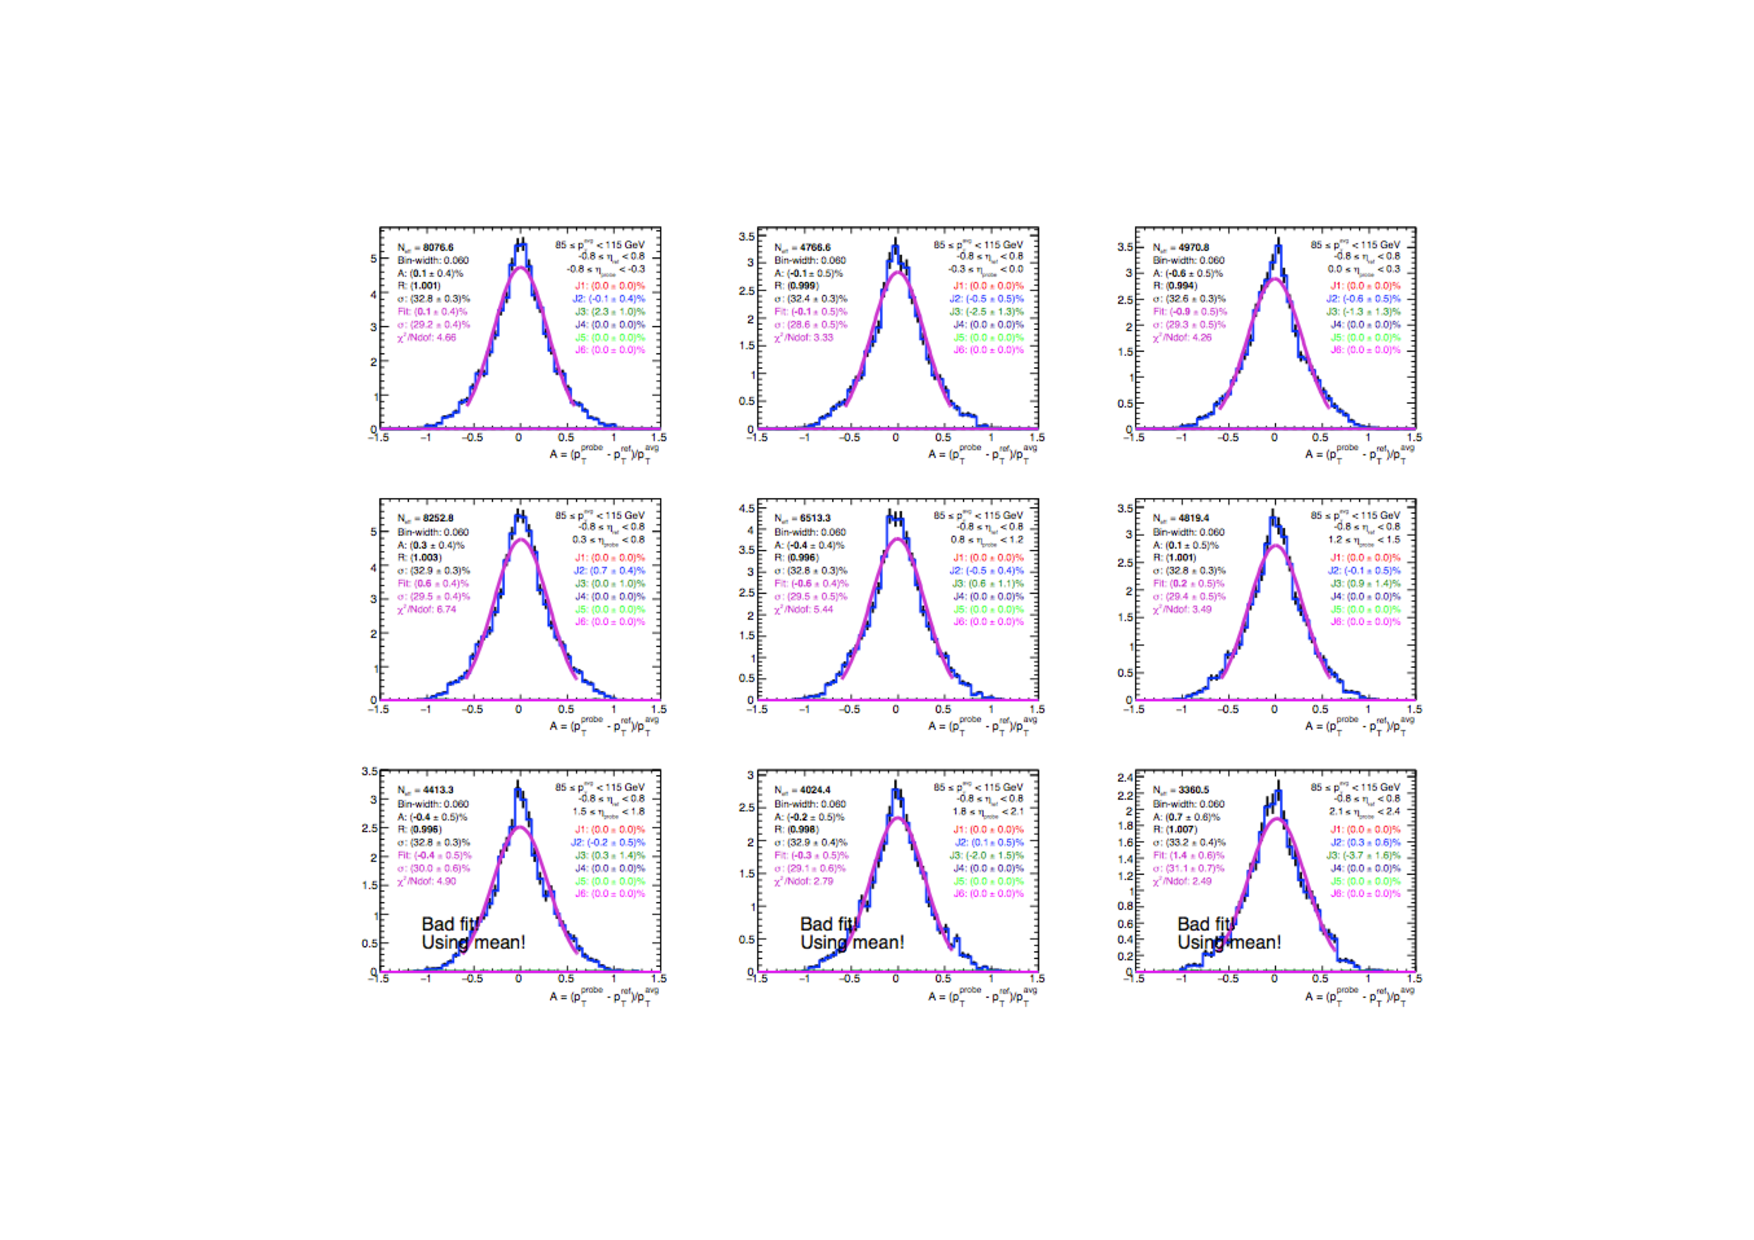
\includegraphics[width=10cm, height=7.5cm]{85to115STruthFitsNoRestrict1.pdf}
\end{frame}

\begin{frame}
\frametitle{Sherpa Truth: After restriction to fit}
\center
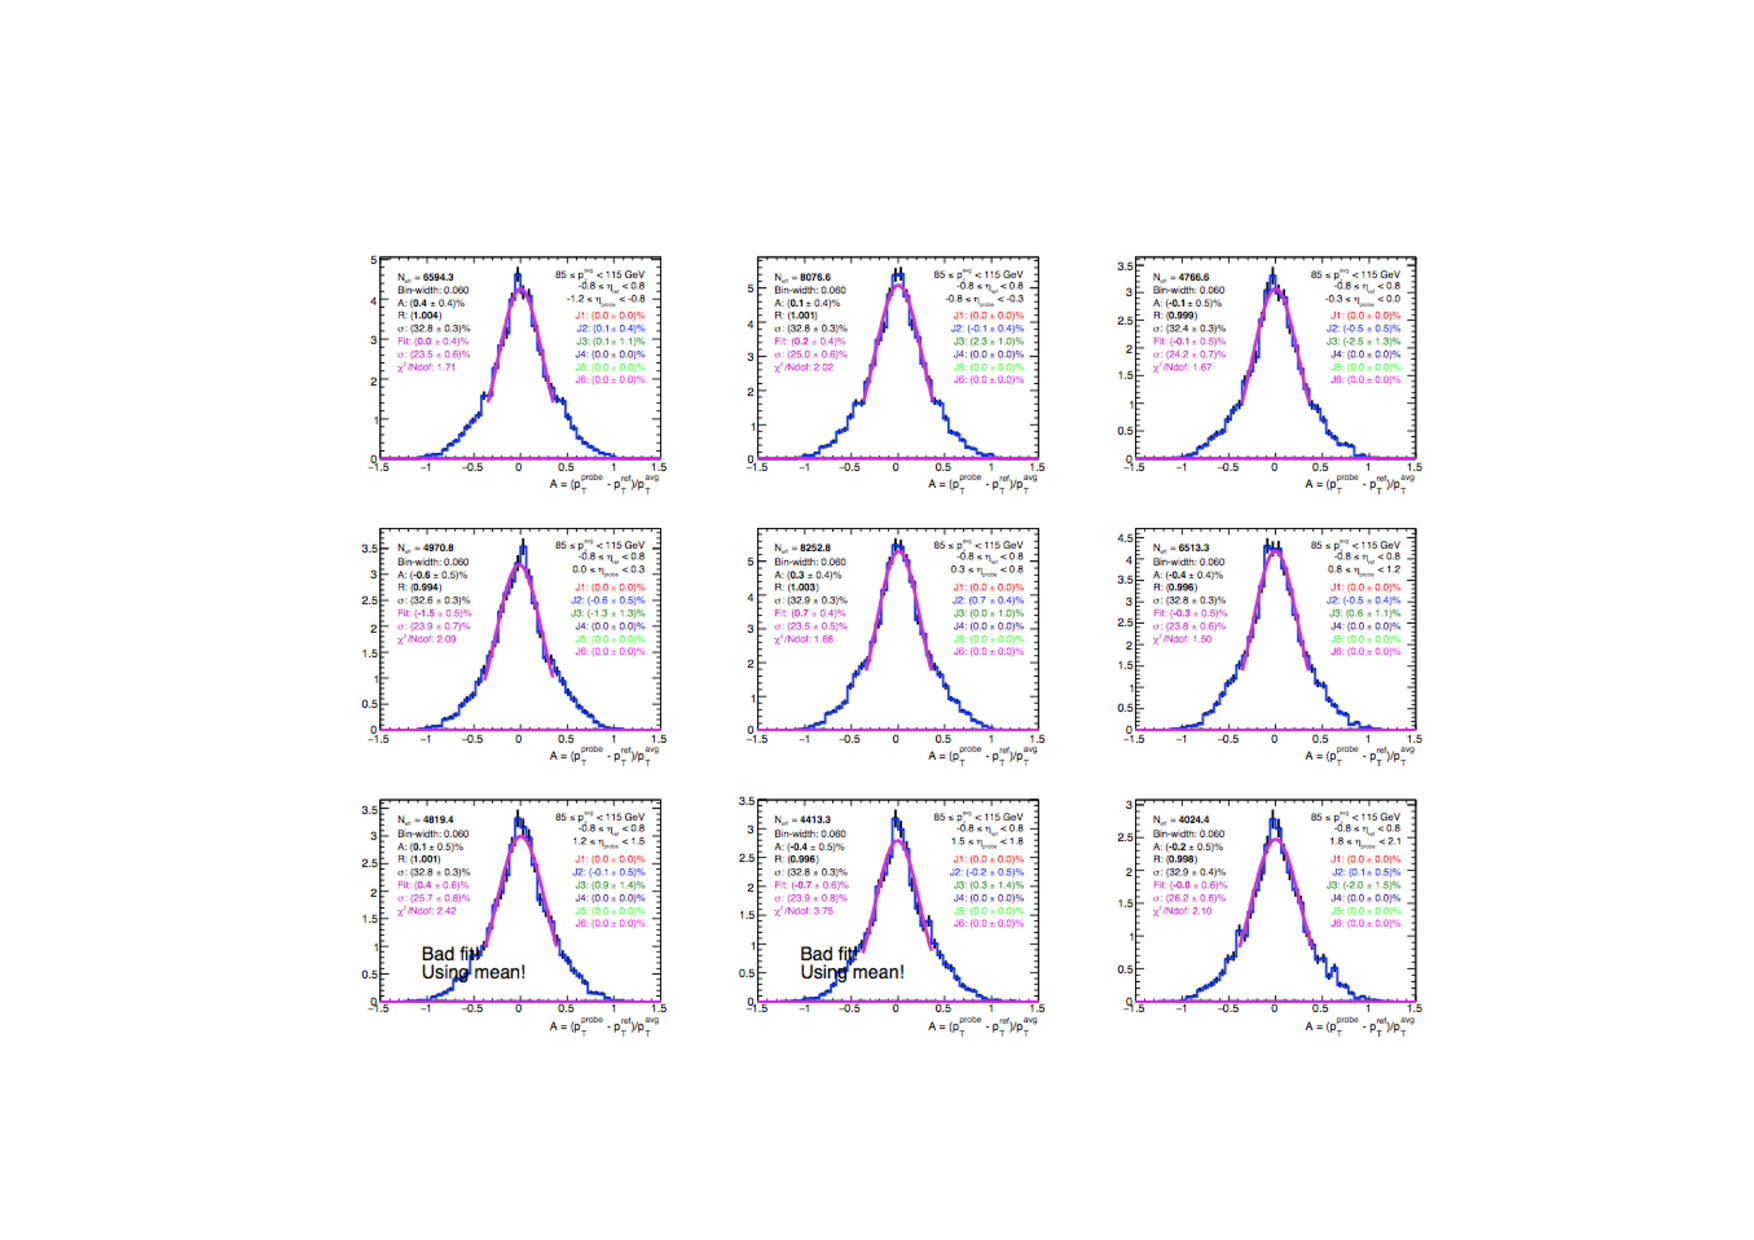
\includegraphics[width=10cm, height=7.5cm]{85to115STruthFits0415_1.pdf}
\end{frame}

\begin{frame}
\frametitle{Sherpa Reco: Before any restrictions}
\center
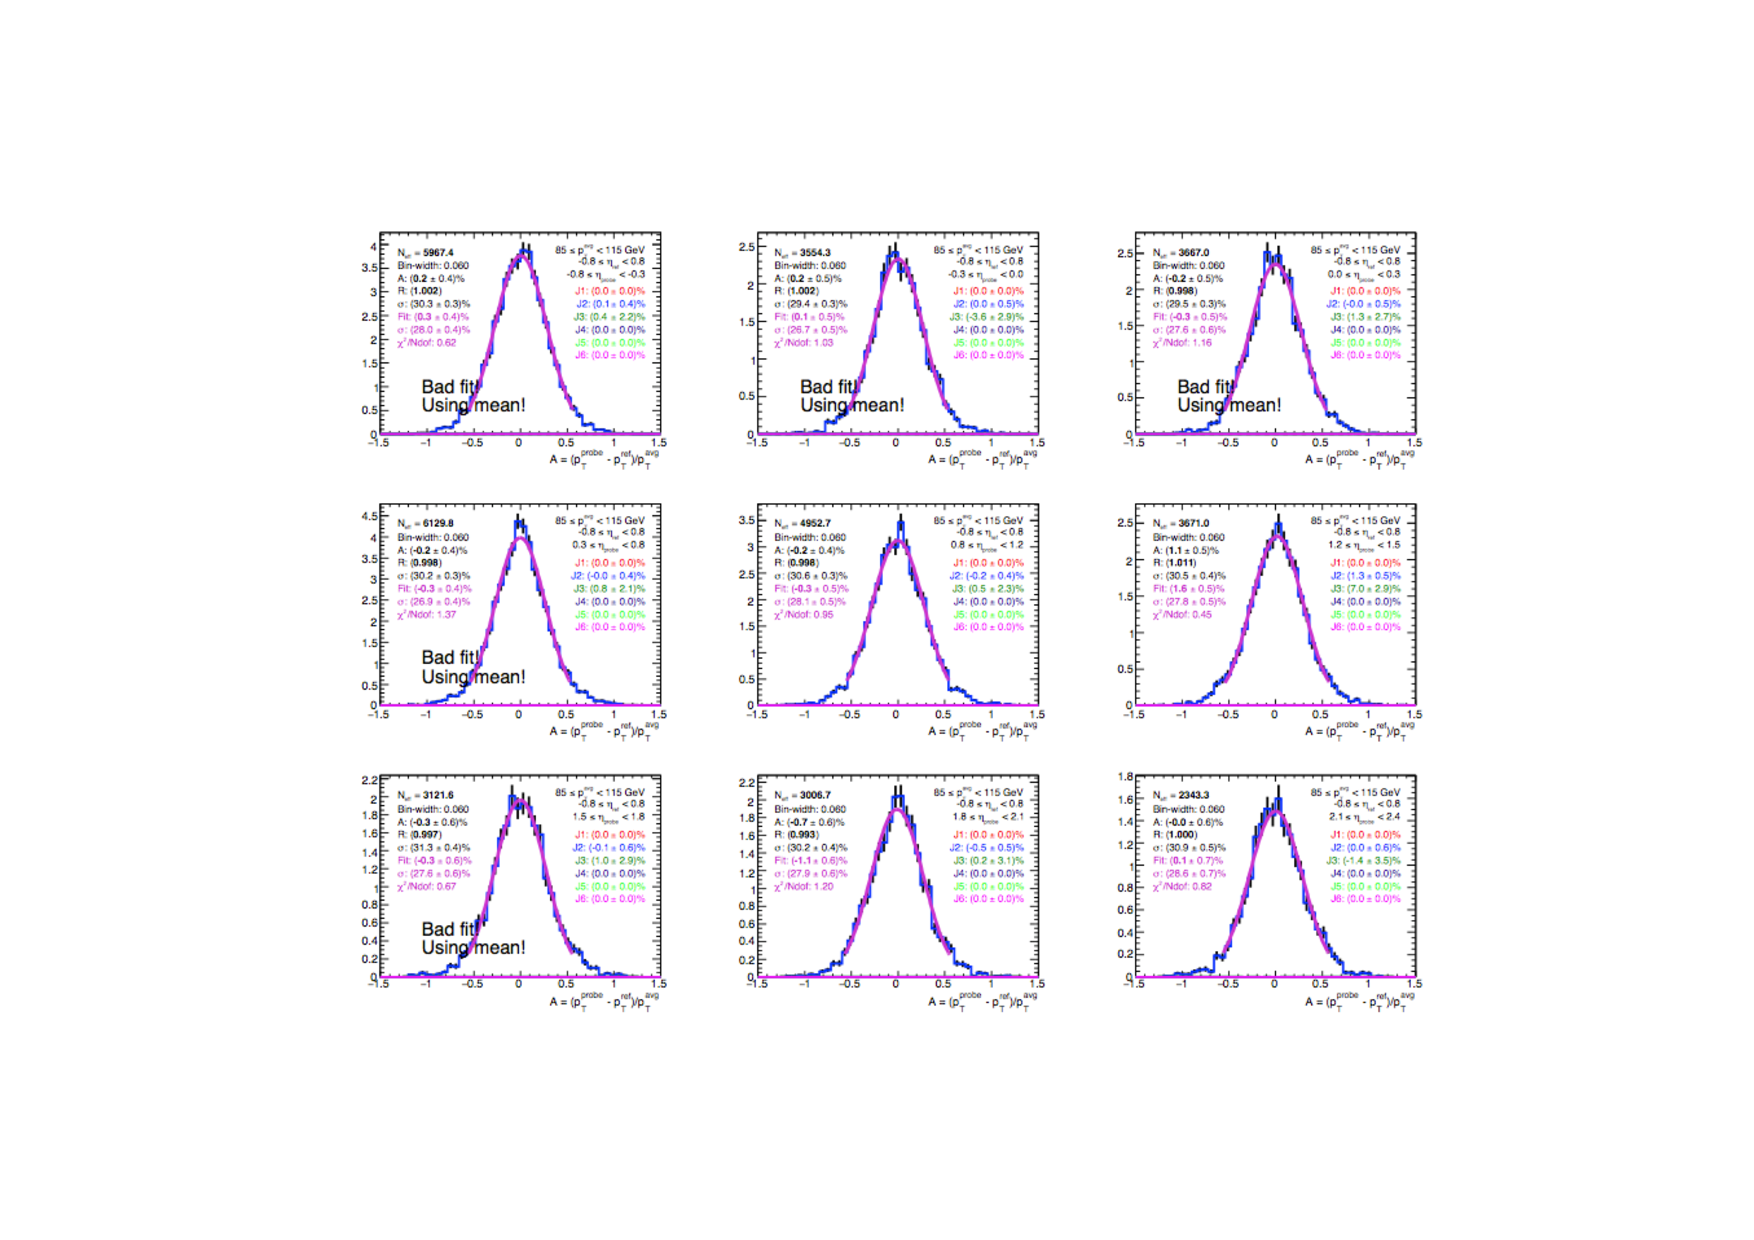
\includegraphics[width=10cm, height=7.5cm]{85to115SRecoFitsNoRestrict1.pdf}
\end{frame}

\begin{frame}
\frametitle{Sherpa Reco: After restriction to fit}
\center
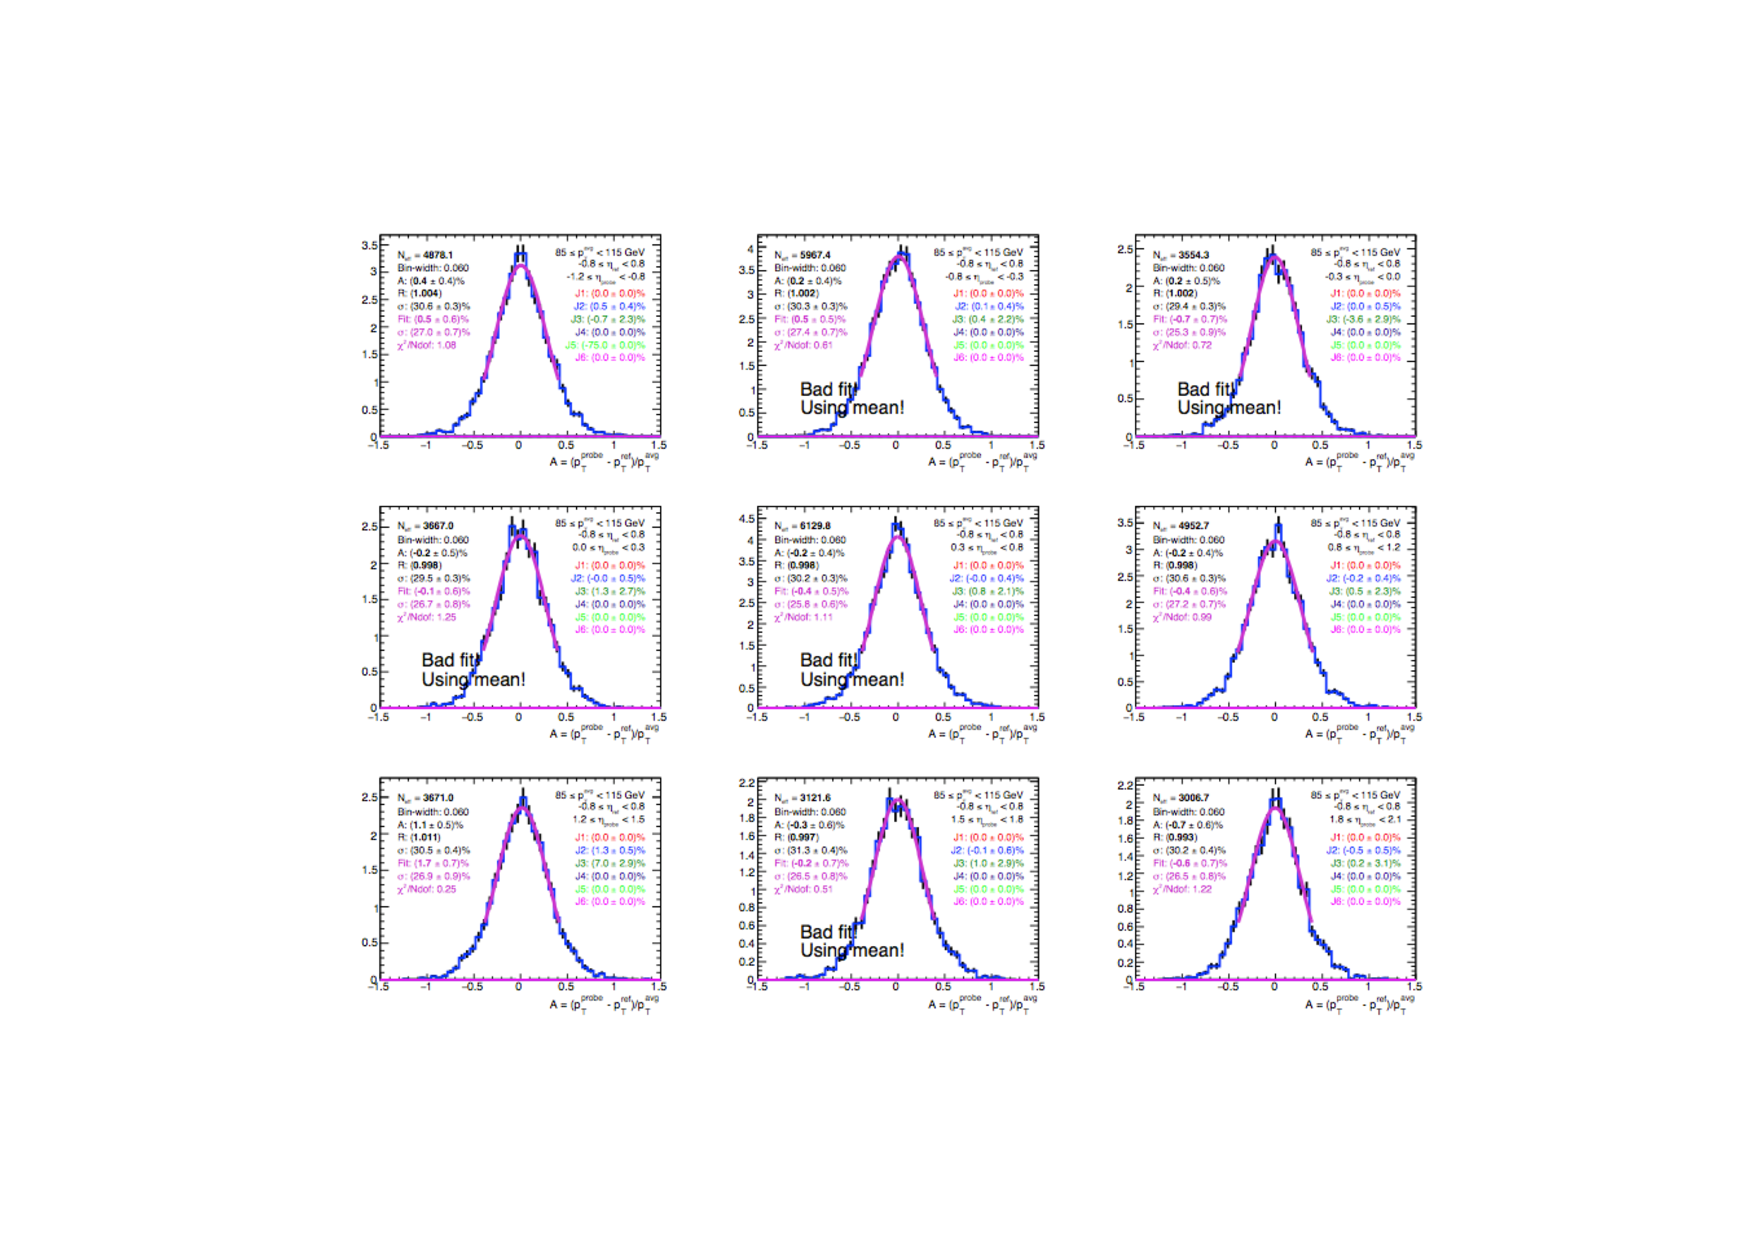
\includegraphics[width=10cm, height=7.5cm]{85to115SRecoFits0415_1.pdf}
\end{frame}

\begin{frame}
\frametitle{Sherpa unsubtracted $\sigma$($P_{T}$)/$P_{T}$ vs $\eta_{det}$ with restrictions}
\begin{columns}
\begin{column}{.4\textwidth}
\includegraphics[width=4.5cm, height=3cm]{MCvsData_Sherpa/25pTavg40_MCvsData.pdf}
\newline
\includegraphics[width=4.5cm, height=3cm]{MCvsData_Sherpa/145pTavg175_MCvsData.pdf}
\end{column}
\begin{column}{.4\textwidth}
\includegraphics[width=4.5cm, height=3cm]{MCvsData_Sherpa/220pTavg270_MCvsData.pdf}
\newline
\includegraphics[width=4.5cm, height=3cm]{MCvsData_Sherpa/270pTavg330_MCvsData.pdf}
\end{column}
\end{columns}
A much smaller number of eta bins of truth are higher than Reco after the fit restriction.
\end{frame}

\begin{frame}
\frametitle{Sherpa unsubtracted $\sigma$($P_{T}$)/$P_{T}$ vs $P_{T}$ with restrictions}
\begin{columns}
\begin{column}{.4\textwidth}
\includegraphics[width=4.5cm, height=3cm]{MCvsData_Sherpa/etaBin3_MCvsData.pdf}
\newline
\includegraphics[width=4.5cm, height=3cm]{MCvsData_Sherpa/etaBin6_MCvsData.pdf}
\end{column}
\begin{column}{.4\textwidth}
\includegraphics[width=4.5cm, height=3cm]{MCvsData_Sherpa/etaBin12_MCvsData.pdf}
\newline
\includegraphics[width=4.5cm, height=3cm]{MCvsData_Sherpa/etaBin19_MCvsData.pdf}
\end{column}
\end{columns}
\end{frame}

\begin{frame}
\frametitle{Sherpa $\sigma$($P_{T}$)/$P_{T}$}
\begin{columns}
\begin{column}{.4\textwidth}
\includegraphics[width=4.5cm, height=3cm]{Difference_Sherpa/25pTavg40_Difference.pdf}
\newline
\includegraphics[width=4.5cm, height=3cm]{Difference_Sherpa/145pTavg175_Difference.pdf}
\end{column}
\begin{column}{.4\textwidth}
\includegraphics[width=4.5cm, height=3cm]{Difference_Sherpa/220pTavg270_Difference.pdf}
\newline
\includegraphics[width=4.5cm, height=3cm]{Difference_Sherpa/270pTavg330_Difference.pdf}
\end{column}
\end{columns}
\begin{itemize}
\item There seems to be an issue with the line connecting points here (Working on it).
\end{itemize}
\end{frame}

\begin{frame}
\frametitle{To-Do:}
\begin{itemize}
\item Continue to fix bug with DeltaR matching to check if this is the problem.
\begin{itemize}
\item Find reason behind truth being larger than reco if matching doesn't fix the problem.\newline
\end{itemize}
\item Fix bugs in code causing lack of connecting points.\newline
\item Start looking at the bisector method.
\end{itemize}
\end{frame}




\end{document} 